% !TEX root=../main.tex
\chapter{Introduction}
\renewcommand{\baselinestretch}{\mystretch}
\label{chap:Intro}
%\setlength{\parindent}{0pt}
\PARstart{P}{rotecting} wild endangered species has become a serious task for local government. GPS tracking and acoustic recording are main techniques to study animals' behaviour~\cite{sueur2012global}. However, It is a time-consuming effort to passively investigate animal's activity.
This report will introduce a method by using deep learning network to automatically detect the acoustic activity of the Geoffroy’s spider monkey. In this chapter, the motivation of this project is firstly discussed. Then, the reasons for choosing deep learning will be introduced in section 1.2. Finally, the organisation and aims will be presented in the last section.
\section{Motivation}
With the rapid development of urbanisation and increasing demands of woods, the biodiversity faces a challenge which needs to be protected especially in tropical rainforest habitats~\cite{soga2014land,wright2006uncertain}. Behaviour analysis is a necessary part in order to not only study biological evolution but also designate nature reserves reasonably. One of the aspects is animal communication, which consists of the transmission of information conveys signals among animals~\cite{green1979analysis}. These acoustic features, such as predator alarm, defending territories or attracting females~\cite{seyfarth2003signalers}, provide a large amount of evidence to study animals' behaviour. Moreover, the organisms whose major components of daily communication is vocalization are suited to apply acoustic monitoring rather than observing or tracking each individual. As Stevenson et al. stated~\cite{stevenson2015general}, acoustic monitoring has advantages of efficient, cost-saving and non‐invasive, compared with the GPS tracking of individuals. \par
There are two types of acoustic monitoring, namely passive and active observation. Passive acoustic monitoring (PAM) is based on fixing recording devices on survey areas, such as installing microphones, hydrophones or others~\cite{kalan2015towards}, to remotely collect acoustic data emitted by animals for a long time period. These are several advantages which make the PAM technique as a preferred method to survey animals. Firstly, acoustic monitoring is cost-saving and energy-efficient compared with other techniques~\cite{mellinger2007overview}. 
Most of the current methods are expensive and require complex systems for aerial imagery, bio‐telemetry and GPS tracking ~\cite{hill2018audiomoth}. With employing low-energy microcontroller, an acoustic device called AudioMoth were developed with benefits of portability and longevity. Due to the reduction in cost from hundreds of dollars to approximately 40 dollars per unit, large-scale and long-term surveys are possible to carry out with a limited budget. \par
Moreover, the acoustic devices are robust to the environment, which can continuously work at night, underwater and other severe conditions. Some groups of organisms, such as cetaceans and primates, are impractically to observe and tracking individuals depending on their submarine or rainforest habitats.
Another distinction of acoustic monitoring is non-invasive property. The acoustic data can be remotely collected with minimal human disturbance due to autonomous units~\cite{kalan2015towards}. Thus, the acoustic record can present animal behaviours in a natural state to a large extent. As a result, acoustic monitoring reduces the detection bias~\cite{alldredge2007time}.\par
Nevertheless, although the PAM technique presents large potentials in investigating animal activity and density, it is a significant challenge to manage and analyse these large data~\cite{Villanueva-RiveraLuisJ.2012PAWM}. Due to passively recording, the autonomous units will continuously work day and night, resulting in terabytes of data saved in the storage. Thus, it will spend a large amount of time for an expert to analysing and labelling the audio with sections of interest. Moreover, the manual observation of calls based on their previous experience can lead to behaviour information being missed and introduce bias at this stage~\cite{digby2013practical}. Hence, a strong motivation with combined techniques from machine learning has been proposed, in which algorithms are designed to automatically detect target sections. 

\section{Deep Learning on Audio data}
Machine learning (ML) technology has explosively improved in recent year, powering many aspects of modern society. The basic learning algorithms, such as support vector machine (SVM), random forests (RF), and Bayesian network, have been successfully applied on classification problems~\cite{sun2009classification}. However, conventional shallow machine learning techniques have limited performance when dealing with raw natural data. Thus, relevant field expertises are necessary to design feature extractor which can describe the raw data in vector representations~\cite{lecun2015deep}. As a consequence, deep learning has been developed with the advantage of multiple levels of representation which are extracted from lower layers~\cite{zhang2018survey}. Therefore, deep learning technique can learn significant features even from raw input data layer by layer and train a classifier at the same time. Furthermore, the coming age of big data makes deep learning evolve rapidly. Depending on high volumes and a large variety of data, deep learning has the capability to effectively and sufficiently learn for classification~\cite{chen2014big}.

However, deep learning is time-cost effort since it needs to not only extract features from a large amount of data to optimize but also train the classifier to solve recognition, detection or classification problems. With the utilisation of powerful GPUs and cloud service~\cite{bao2018scalable}, the neural network with high computational complexity can be trained to acquire impressive performance. Convolutional neural network (CNN) is one of the extensive networks based on deep learning, which has an outstanding performance on image analysis. CNN has been utilised in many situations, such as video event detection \cite{xu2015discriminative}, face recognition~\cite{parkhi2015deep}, audio classification~\cite{lee2009unsupervised}. Moreover, changing model architecture can focus on the different target in order to improve performance. CNN highly impressed people in image recognition when AlexNet was introduced with champion performance in 2012 ImageNet competition~\cite{krizhevsky2012imagenet}. Afterwards, performances were improved along with VGGNet~\cite{simonyan2014very} and GoogleNet~\cite{43022}. Fast R-CNN~\cite{girshick2015fast} was proposed to efficiently classify objects. In addition, residual learning with 152 layers ResNet was proposed to solve hard training problem in very deep layer architecture~\cite{he2016deep}.\par
\begin{figure}[htp]
  \centering
  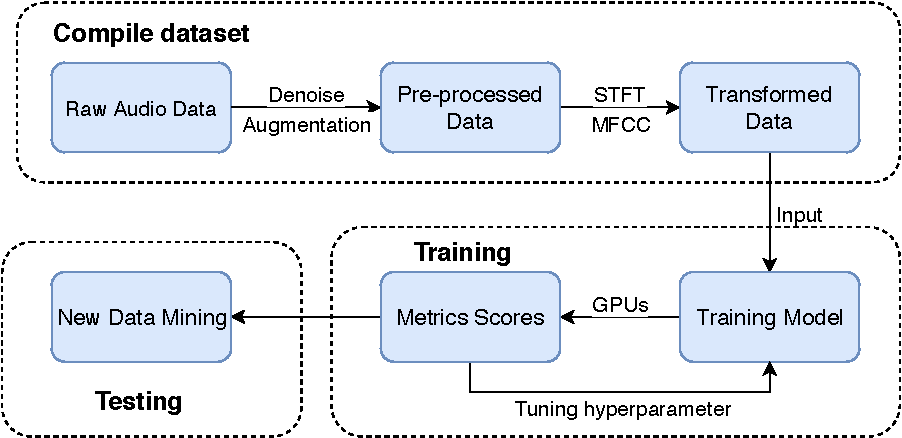
\includegraphics[scale=1]{Figs/intro/pipline.pdf}
  \caption{General steps of deep learning on audio data}
  \label{Fig:pipline}
\end{figure}
Audio as one of the data types has been developed as well. Via transforming time-series audio data into spectrograms, CNN can be applied to learn audio data based on spectral analysis. Fig.\ref{Fig:pipline} depicts the general steps of audio data detection in deep learning. There are three main procedures in audio data learning. First, the raw audio data need to apply signal processing methods for several purposes like denoising, clipping and augmentation. Afterwards, the time-series data are transformed into spectrograms as the input of CNNs model. Short-Time Fourier Transform (STFT) and Mel-Frequency Cepstral Coefficients (MFCC) are effective feature extraction techniques, transforming temporal characteristics into the spectral domain. During model training, different metrics are used to evaluate the performance, which is significant in tuning hyperparameters. If the model is fine-tuned, we can mine new data with significant accuracy. 

\section{Data Collection}
In this project, the audio data were recorded of endangered tropical primate Geoffroy's spider monkey, \textit {Ateles geoffroyi}. This species is significantly suitable for analysis since they highly depend on vocalized communication. With large contributions of Miss. Jenna Lawson who is a PhD student researching in Life Sciences, the raw audio data were labelled in an appropriate way. The spider monkey calls were collected by AudioMoth recording devices at a 48 kHz sampling rate, installed on the Osa Peninsula. This device generates minute-long files in \text{'.wav'} format and named by a hexadecimal code which represents the recording date and time. \par
In details with explanation by Jenna, there are 360 audio locations, each recording for 7 days, totals 36,800 hours of acoustic data over 2520 days of recording. Fig~\ref{fig:locations} demonstrates the habitat types and levels of protection audio data were found in, including 3 national parks, a reserve and unprotected regions on the Osa Peninsula of Costa Rica. It took one year to collect all the data and an additional 3 months of pilot studies to ensure that the spider monkeys actually make enough sounds to work and to test out the audio equipment. However, it is the most challenging effort to find the calls from the pilot data. Due to the rarity of spider monkey, only 388 presences of call were marked in 900 hours data, resulting in a small training dataset. Moreover, it took 30 more hours to record the positions in to 'Praat file'. Hence, the automated detection system is significantly necessary.

\begin{figure}[htp]
\centering
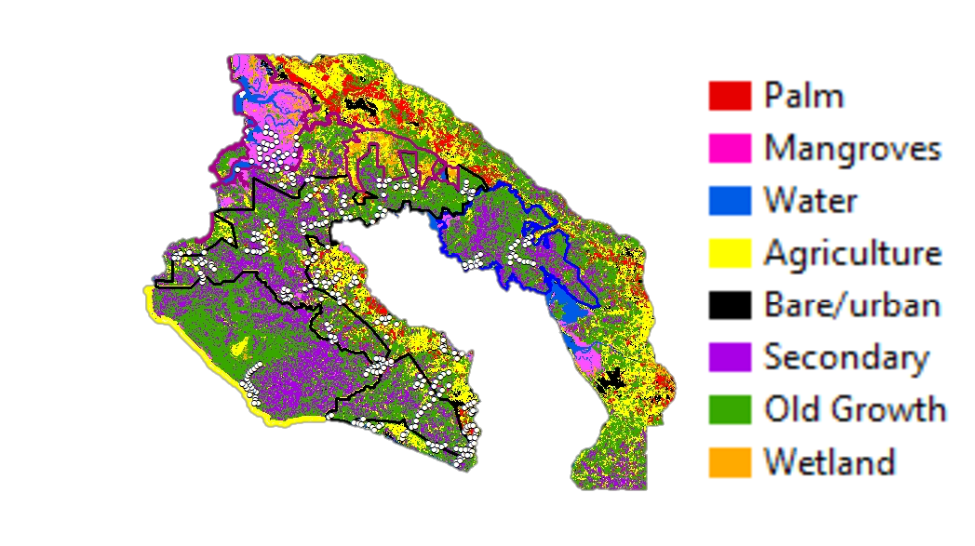
\includegraphics[scale=0.8]{Figs/intro/locations.pdf}
\caption{Locations of Osa Peninsula in Costa Rica (provided by Jenna)}
\label{fig:locations}
\end{figure}

\section{Aims and Organisation}
As a case study, this project is purposed to design and improve an automated detection system based on Deep Learning. The objectives are shown below:
\begin{itemize}
\item Pre-process the raw audio data into appropriate segments in order to extract the features effectively. Depending on mel-spectrogram of frequencies varying with time, compile the training and testing data. We aim to apply augmentation and denoising algorithms to evaluate performance.
\item Use self-designed CNN model to train the data as a baseline in a balanced way. Other applied methods of hard-negative-mining, weighted loss in the unbalanced dataset, denoising, and augmentation are as comparisons to evaluate model performance.
\item Use state-of-art like VggNet architectures with same train audio data. If the model is fine-tuning, then the model performance can have large improvement.
\item Use the trained model to predict new test acoustic data. Record and write the model predictions in files for manual check.
\end{itemize}
And the report is divided into six chapters and will be organized as follows:
\begin{itemize}
\item In Chapter 2, a background and literature review of audio data learning will be presented with parts of feature extraction and several studies of deep learning applied on audio data.
\item In Chapter 3, the methodology of pre-processing methods and basic theory of CNN will be introduced, including feature extraction, layers, the learning process of CNN, denoising and augmentation. The reasons for the chosen layers and loss function will be explained.
\item Chapter 4 will describe the implementation of this project and discuss the performance with evaluated metrics.
\item In Chapter 5 and 6, a summary will be presented of this project, following with the inspirations of future works.
\end{itemize}

